\chapter{Fundamentação Teórica}

\section{Persistência Poliglota}

\citeonline{ford2008productive} introduziu o conceito de ``programação poliglota'' para
expressar a ideia de que aplicativos devem ser desenvolvidos utilizando uma combinação de
linguagens, aproveitando o fato de que diferentes linguagens são mais adequadas para lidar
com diferentes problemas. Uma das consequências notáveis da programação poliglota é a
transição para a ``persistência poliglota'', usando a mesma analogia: pode-se dizer que
múltiplas tecnologias de bancos de dados podem ser utilizadas como armazenamento
persistente para diferentes tipos de casos de uso. Embora ainda exista uma quantidade
considerável de dados gerenciados por sistemas relacionais, a abordagem predominante passa
a ser a reflexão sobre como se deseja manipular os dados antes de determinar qual tecnologia
é a mais adequada para essa manipulação \cite{fowler2011polyglot}.

A persistência poliglota abrange uma variedade de formatos de dados, incluindo
estruturados, semi-estruturados e não estruturados. Dados estruturados geralmente englobam
formatos como relacional, objeto-relacional, e grafos de propriedades. Dados
semi-estruturados incluem principalmente documentos JSON e XML. Por fim, dados não
estruturados são representados por arquivos de texto, imagens e áudios, dentre outros
\cite{ye2023benchmark}.

Um domínio em que a persistência poliglota pode ser aplicada é o de um e-commerce. Nesse
cenário, diferentes categorias de dados possuem características e padrões de acesso
distintos --- volume de escrita, frequência de leitura, necessidade de consistência,
estrutura dos registros --- o que torna mais adequado o uso de um SGBD específico para
cada uma delas. A Figura~\ref{fig:polyglot-ecommerce} ilustra esse cenário, mapeando cada
categoria de dado do e-commerce ao SGBD mais adequado, conforme sugerido a seguir:

\begin{figure}[H]
  \centering
  \caption{Exemplo de aplicação da Persistência Poliglota em um e-commerce.}
  \label{fig:polyglot-ecommerce}
  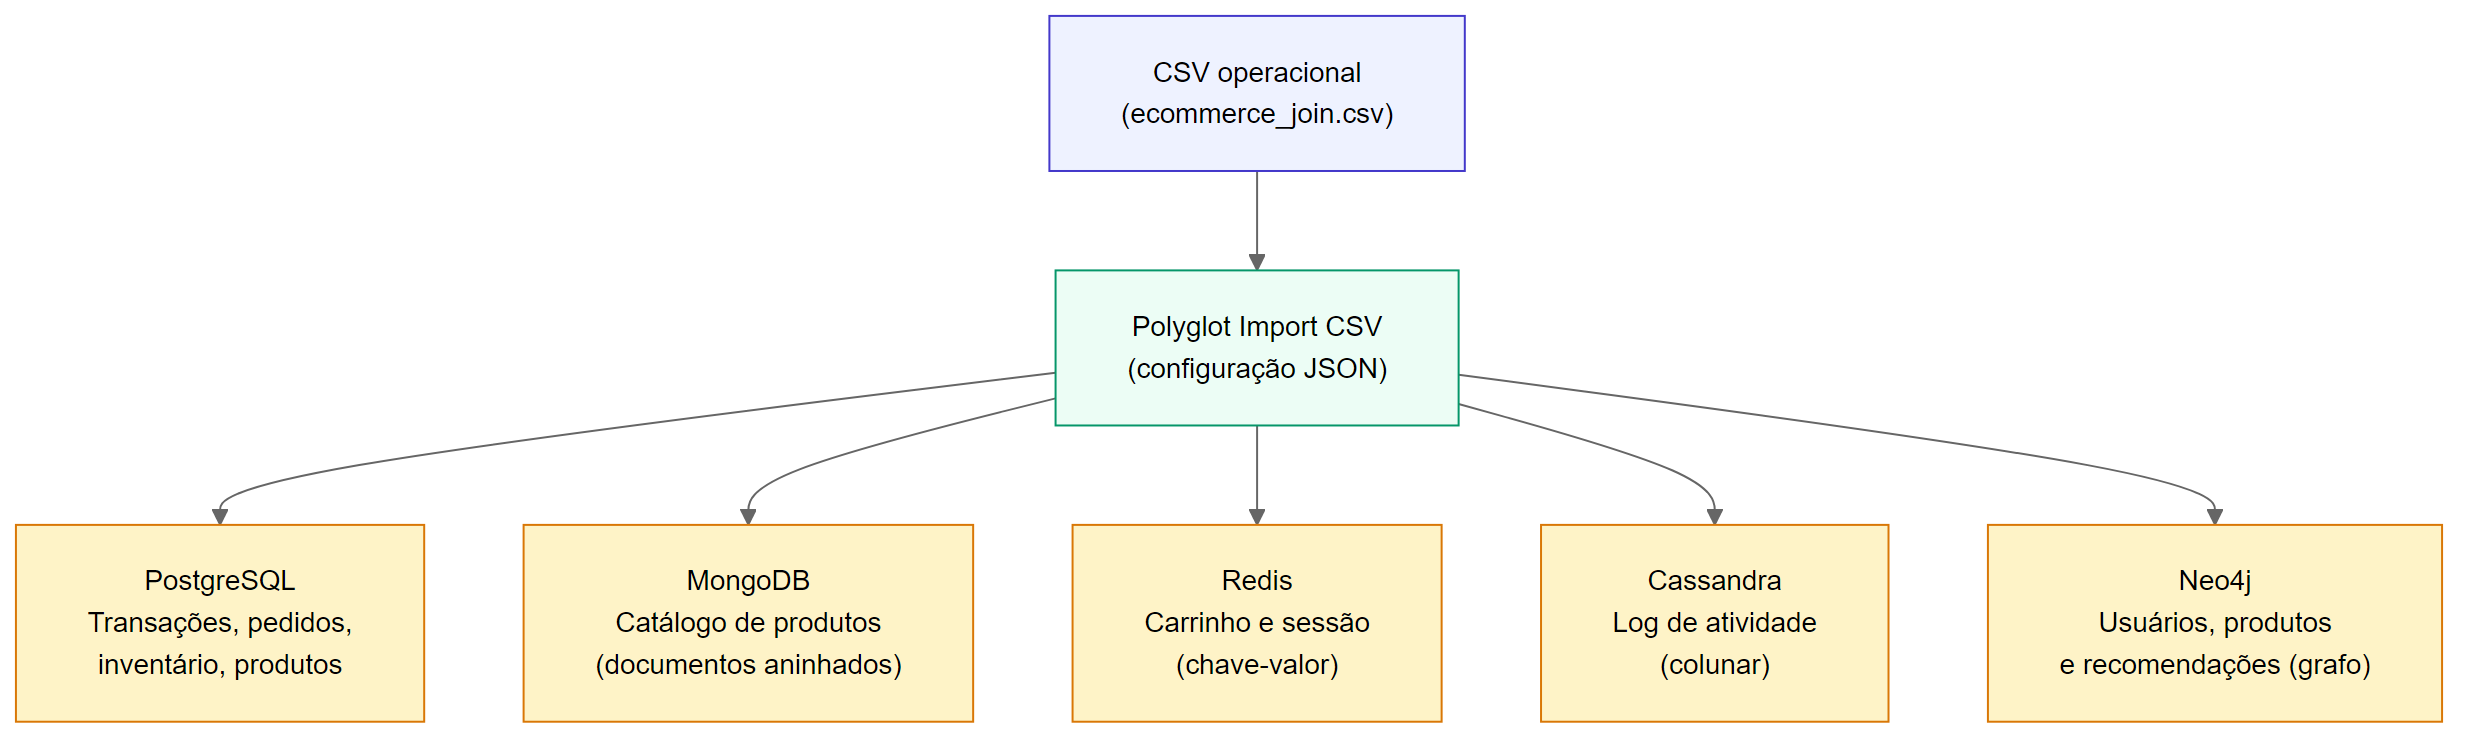
\includegraphics[width=15cm]{images/figure1-polyglot-ecommerce}
  \par\vspace{4pt}
  {\footnotesize Fonte: Elaborado pelo autor (2026).}
\end{figure}

\begin{itemize}
  \item \textbf{Dados Financeiros/Transacionais de Pagamento e Inventário de Produtos:}
  Pedidos, pagamentos e estoques exigem garantias transacionais fortes (ACID) para evitar
  inconsistências --- por exemplo, debitar um pagamento sem registrar o pedido
  correspondente. Além disso, consultas analíticas sobre esses dados frequentemente
  combinam várias entidades por meio de junções. Bancos de dados relacionais como o
  PostgreSQL são a escolha natural para esse perfil, pois oferecem suporte nativo a
  transações com consistência forte, integridade referencial e uma linguagem de consulta
  expressiva (SQL).

  \item \textbf{Dados do Catálogo de Produtos:} O catálogo de um e-commerce tende a ter
  esquema variável: diferentes produtos possuem atributos distintos (um livro físico com
  ISBN e editora; um eletrodoméstico com voltagem e garantia). Além disso, o catálogo é
  lido com muito maior frequência do que escrito, e cada consulta normalmente recupera o
  produto completo de uma vez. Bancos de dados orientados a documentos como o MongoDB são
  otimizados exatamente para esse perfil: armazenam cada produto como um documento
  autocontido (favorecendo leituras de agregados complexos), suportam esquemas flexíveis e
  oferecem índices secundários e \textit{pipelines} de agregação para fins de consulta.

  \item \textbf{Dados da Sessão e do Carrinho de Compras do Usuário:} Dados de sessão e
  carrinho são acessados a cada interação do usuário durante a navegação, exigindo latência
  mínima, e são também inerentemente temporários --- um carrinho abandonado não precisa
  persistir indefinidamente. Bancos de dados chave-valor em memória como o Redis oferecem
  latência de microssegundos, expiração automática de chaves e são horizontalmente
  escaláveis para absorver picos de tráfego, tornando-se a escolha ideal para dados de
  natureza efêmera e de acesso intenso.

  \item \textbf{Dados de Atividade do Usuário:} Eventos de navegação
  (\textit{clickstream}), visualizações de produto e histórico de ações são gerados em alto
  volume e alta velocidade. Consultas típicas percorrem o histórico de um usuário em um
  intervalo de tempo, ou agregam eventos por tipo de ação. Bancos de dados colunares como o
  Apache Cassandra são projetados para ingestão massiva com particionamento por chave
  primária composta (por exemplo, \texttt{(user\_id, timestamp)}), garantindo escritas
  rápidas e leituras eficientes por usuário ou período --- padrão ideal para séries
  temporais de atividade.

  \item \textbf{Dados de Recomendação:} Sistemas de recomendação dependem de
  relacionamentos entre entidades: usuários que compraram os mesmos produtos, produtos
  frequentemente adquiridos em conjunto ou usuários com perfis semelhantes. Esses padrões
  são naturalmente modelados como grafos, onde nós representam usuários e produtos, e
  arestas representam interações (comprou, avaliou, visualizou, etc.). Bancos de dados
  orientados a grafos como o Neo4j permitem percorrer esses relacionamentos com eficiência
  por meio de consultas Cypher, tarefa que em um banco de dados relacional exigiria
  múltiplas junções e difícil otimização.
\end{itemize}

\section{Bancos de Dados NoSQL}

Os bancos de dados NoSQL podem ser divididos em subcategorias com base em seus modelos de
dados. Este trabalho utiliza a classificação de \citeonline{hecht2011nosql}, que categoriza
os bancos de dados NoSQL em quatro tipos: chave-valor, colunares, documentos e grafos.

A Figura~\ref{fig:nosql-models} ilustra esses modelos de dados, que são detalhados a
seguir.

\begin{figure}[H]
  \centering
  \caption{Diferentes tipos de modelos de dados NoSQL.}
  \label{fig:nosql-models}
  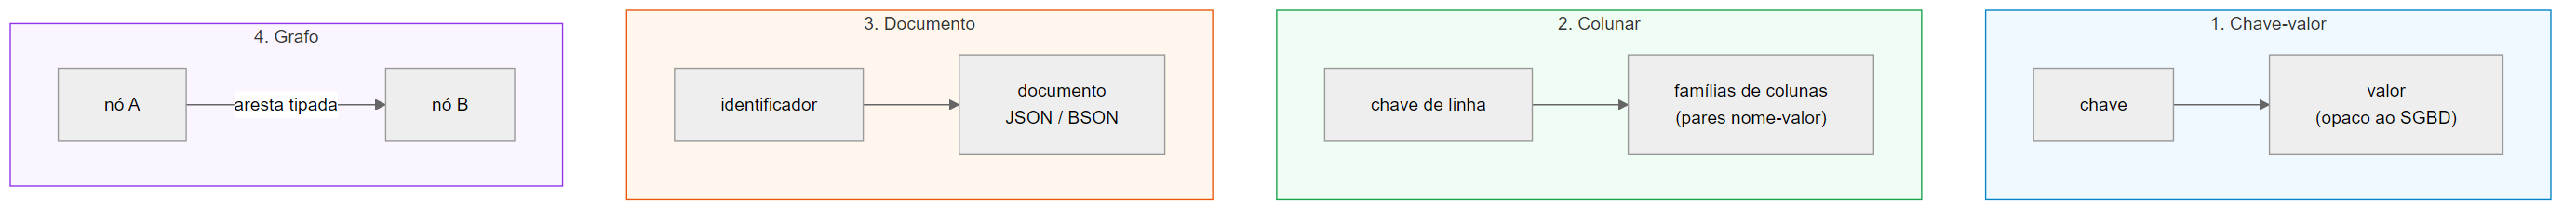
\includegraphics[width=15cm]{images/figure2-nosql-data-models}
  \par\vspace{4pt}
  {\footnotesize Fonte: Elaborado pelo autor (2026).}
\end{figure}

\subsection{Chave-valor}

Os bancos de dados de chave-valor têm um modelo de dados simples baseado justamente em
pares chave-valor, semelhante a um mapa associativo ou dicionário. A chave identifica
exclusivamente o valor e é usada para armazenar e recuperar o valor no banco de dados,
funcionando como uma chave primária. O valor pode ser usado para armazenar qualquer dado
arbitrário, incluindo um número inteiro, uma \textit{string}, um \textit{array} ou um
objeto, proporcionando uma representação de dados sem esquema conhecido.

Além disso, os bancos de dados de chave-valor são muito eficientes no armazenamento de
dados distribuídos, mas não são adequados para cenários que requerem a definição de
relacionamentos entre dados ou esquemas fortemente estruturados. Qualquer funcionalidade
que necessite desses requisitos deve ser implementada na aplicação cliente que interage com
o banco de dados chave-valor.

Como os valores são opacos para os bancos de dados, esses não podem lidar com consultas e
indexações a nível de dados, podendo realizar consultas apenas por meio de chaves. Um
exemplo de SGBD chave-valor é o Redis, que mantém os dados tanto na memória como no disco.
A Figura~\ref{fig:nosql-keyvalue} ilustra o modelo com um exemplo de carrinho de compras
e sessão de usuário, em que cada chave aponta para um valor opaco ao SGBD.

\begin{figure}[H]
  \centering
  \caption{Modelo chave-valor: chaves apontando para valores arbitrários (Redis).}
  \label{fig:nosql-keyvalue}
  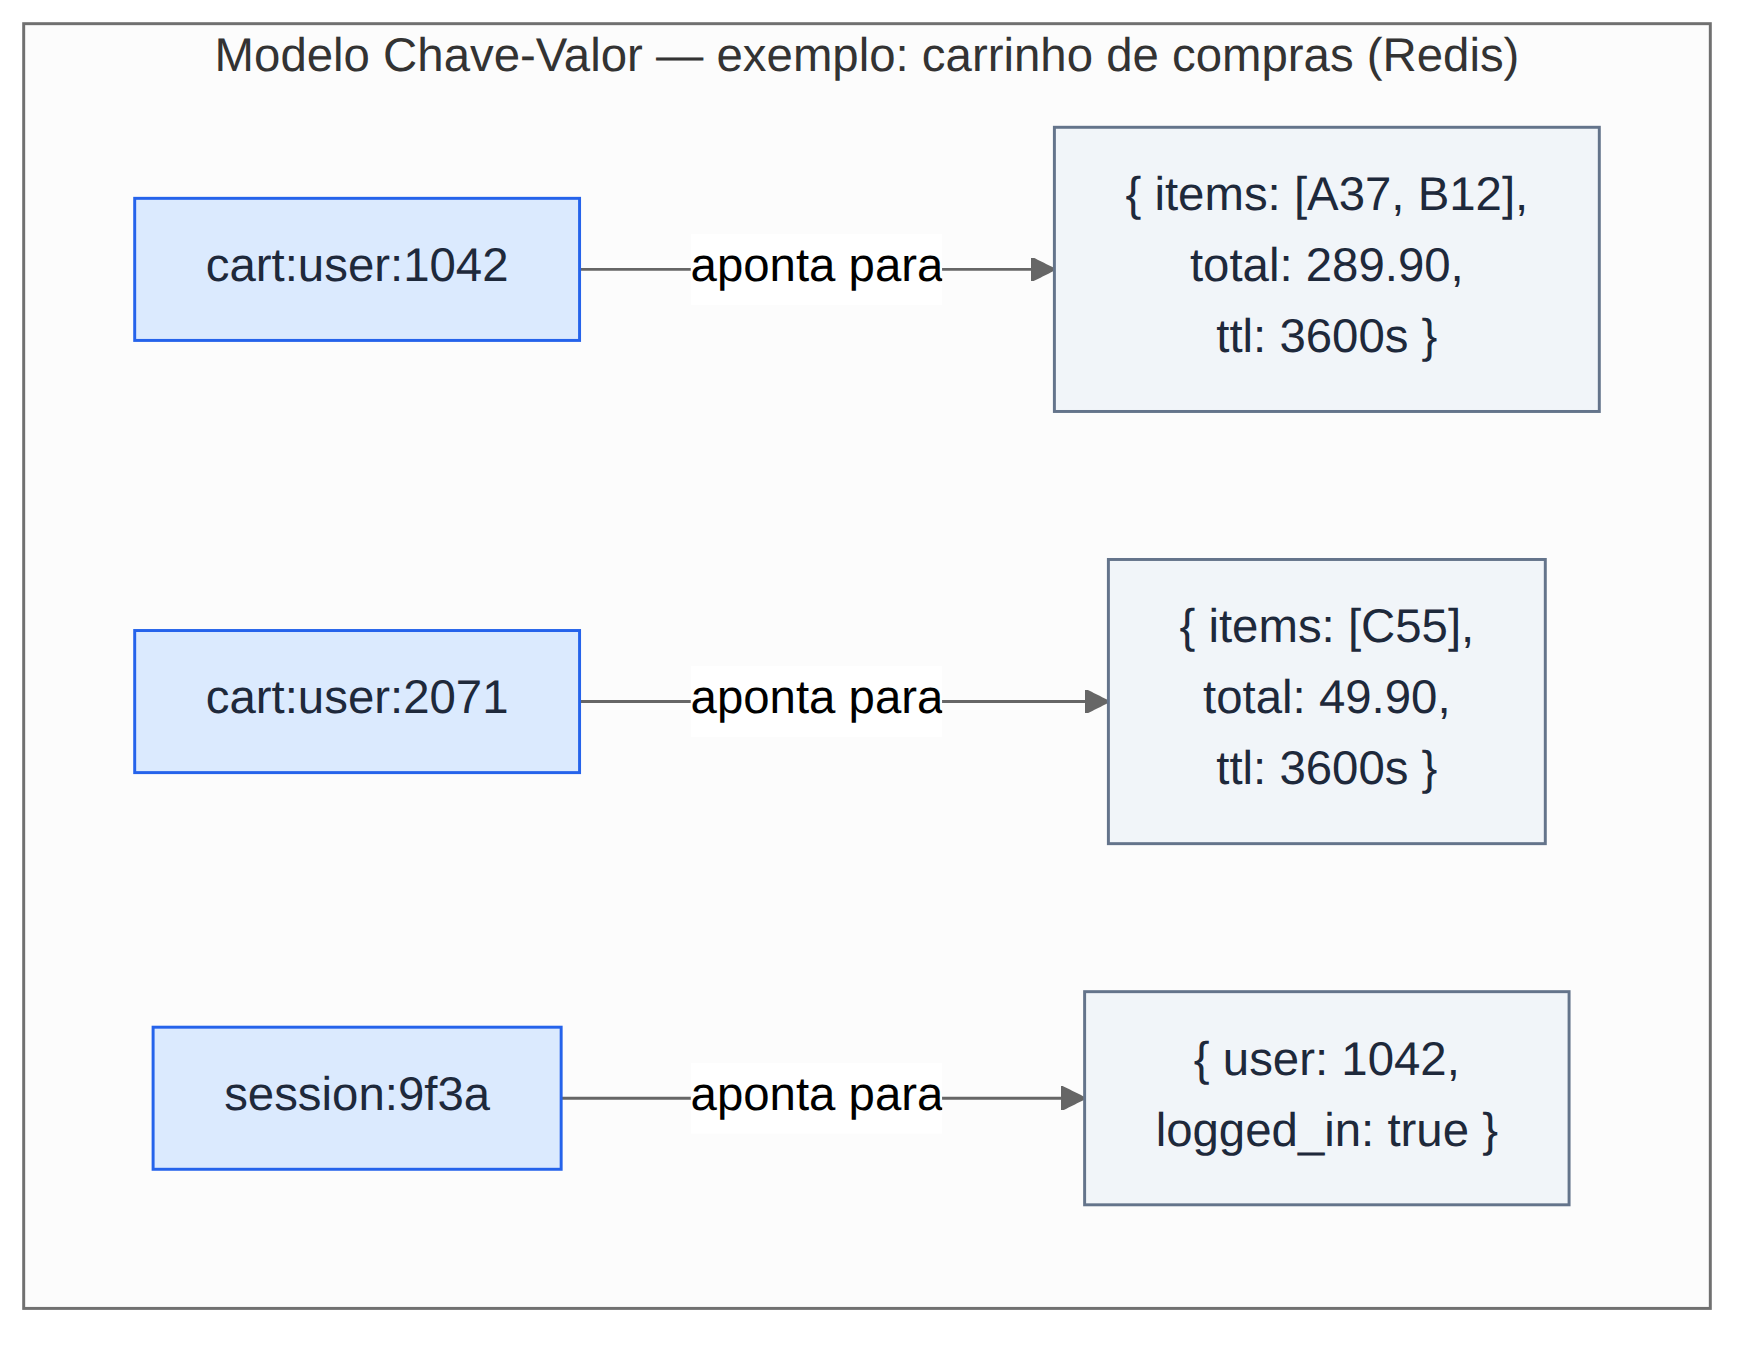
\includegraphics[width=12cm]{images/figure3-nosql-keyvalue}
  \par\vspace{4pt}
  {\footnotesize Fonte: Elaborado pelo autor (2026).}
\end{figure}

\subsection{Colunar}

Em bancos de dados colunares, o conjunto de dados consiste em várias linhas, cada uma
identificada por uma chave de linha única, semelhante a uma chave primária. Cada linha é
composta por uma família (ou conjunto) de colunas, e diferentes linhas podem ter diferentes
famílias de colunas. Semelhante aos bancos de dados de chave-valor, a chave de linha
funciona como a chave, e o conjunto de famílias de colunas atua como o valor representado
pela chave de linha. No entanto, colunas em uma família de colunas consistem em pares
atributo-valor que podem ser indexadas. O SGBD Cassandra oferece a funcionalidade adicional
de supercolunas, que são criadas agrupando várias colunas.

Normalmente, os dados pertencentes a uma linha são armazenados juntos no mesmo nó do
servidor. No entanto, o Cassandra pode distribuir uma única linha por vários nós de
servidor usando chaves de partição compostas. Nos bancos de dados colunares, a configuração
das famílias de colunas é tipicamente feita durante a inicialização. No entanto, a
definição prévia de colunas não é necessária, oferecendo grande flexibilidade no
armazenamento de qualquer tipo de dado.

De forma semelhante aos bancos de dados de chave-valor, qualquer lógica que exija relações
deve ser implementada na aplicação cliente, ou seja, essa categoria de banco de dados
também não têm ciência de relacionamentos entre dados e controle de integridade referencial.
A Figura~\ref{fig:nosql-columnar} apresenta um exemplo de \textit{log} de atividade, em que
cada chave de linha (\texttt{user\_id}) agrupa uma família de colunas com eventos
indexados por \textit{timestamp}.

\begin{figure}[H]
  \centering
  \caption{Modelo colunar: chaves de linha e famílias de colunas (Cassandra).}
  \label{fig:nosql-columnar}
  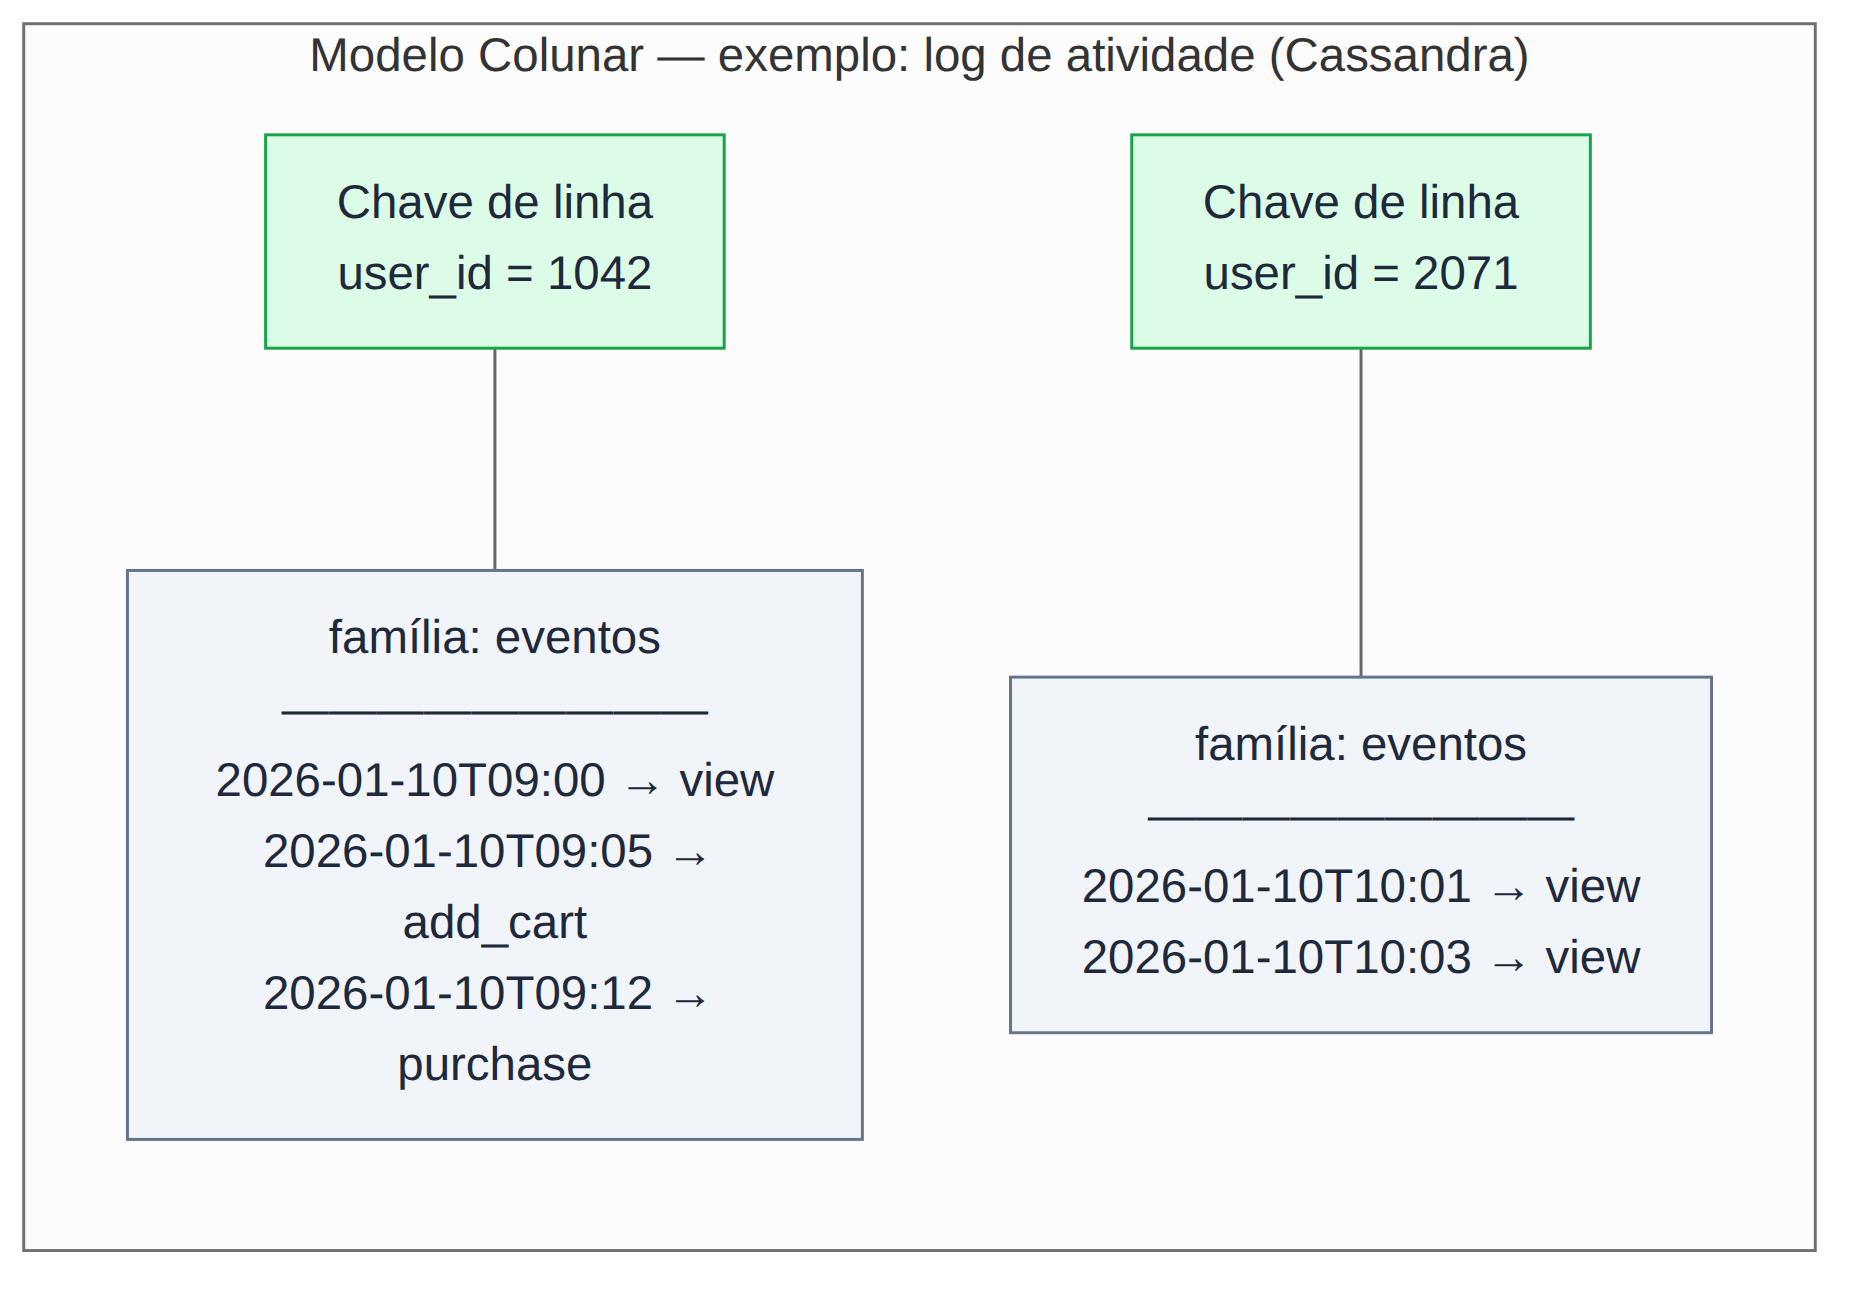
\includegraphics[width=12cm]{images/figure4-nosql-columnar}
  \par\vspace{4pt}
  {\footnotesize Fonte: Elaborado pelo autor (2026).}
\end{figure}

\subsection{Documento}

Bancos de dados orientados a documento armazenam dados como documentos autocontidos, em
geral em formato JSON ou BSON. Cada documento possui um identificador e um conjunto de
campos que podem variar entre documentos de uma mesma coleção, favorecendo esquemas
flexíveis e agregados de leitura (\textit{read-optimized}). O SGBD MongoDB é um exemplo
popular nesta categoria. Ele define coleções de documentos, índices secundários e
\textit{pipelines} de agregação, permitindo consultas ricas sem exigir junções
(\textit{joins}) no servidor. A Figura~\ref{fig:nosql-document} ilustra uma coleção de
catálogo de produtos, em que cada documento é autocontido e pode conter subdocumentos
aninhados (como \texttt{category} e \texttt{stock}) e campos distintos entre si.

\begin{figure}[H]
  \centering
  \caption{Modelo de documento: documentos autocontidos com campos variáveis (MongoDB).}
  \label{fig:nosql-document}
  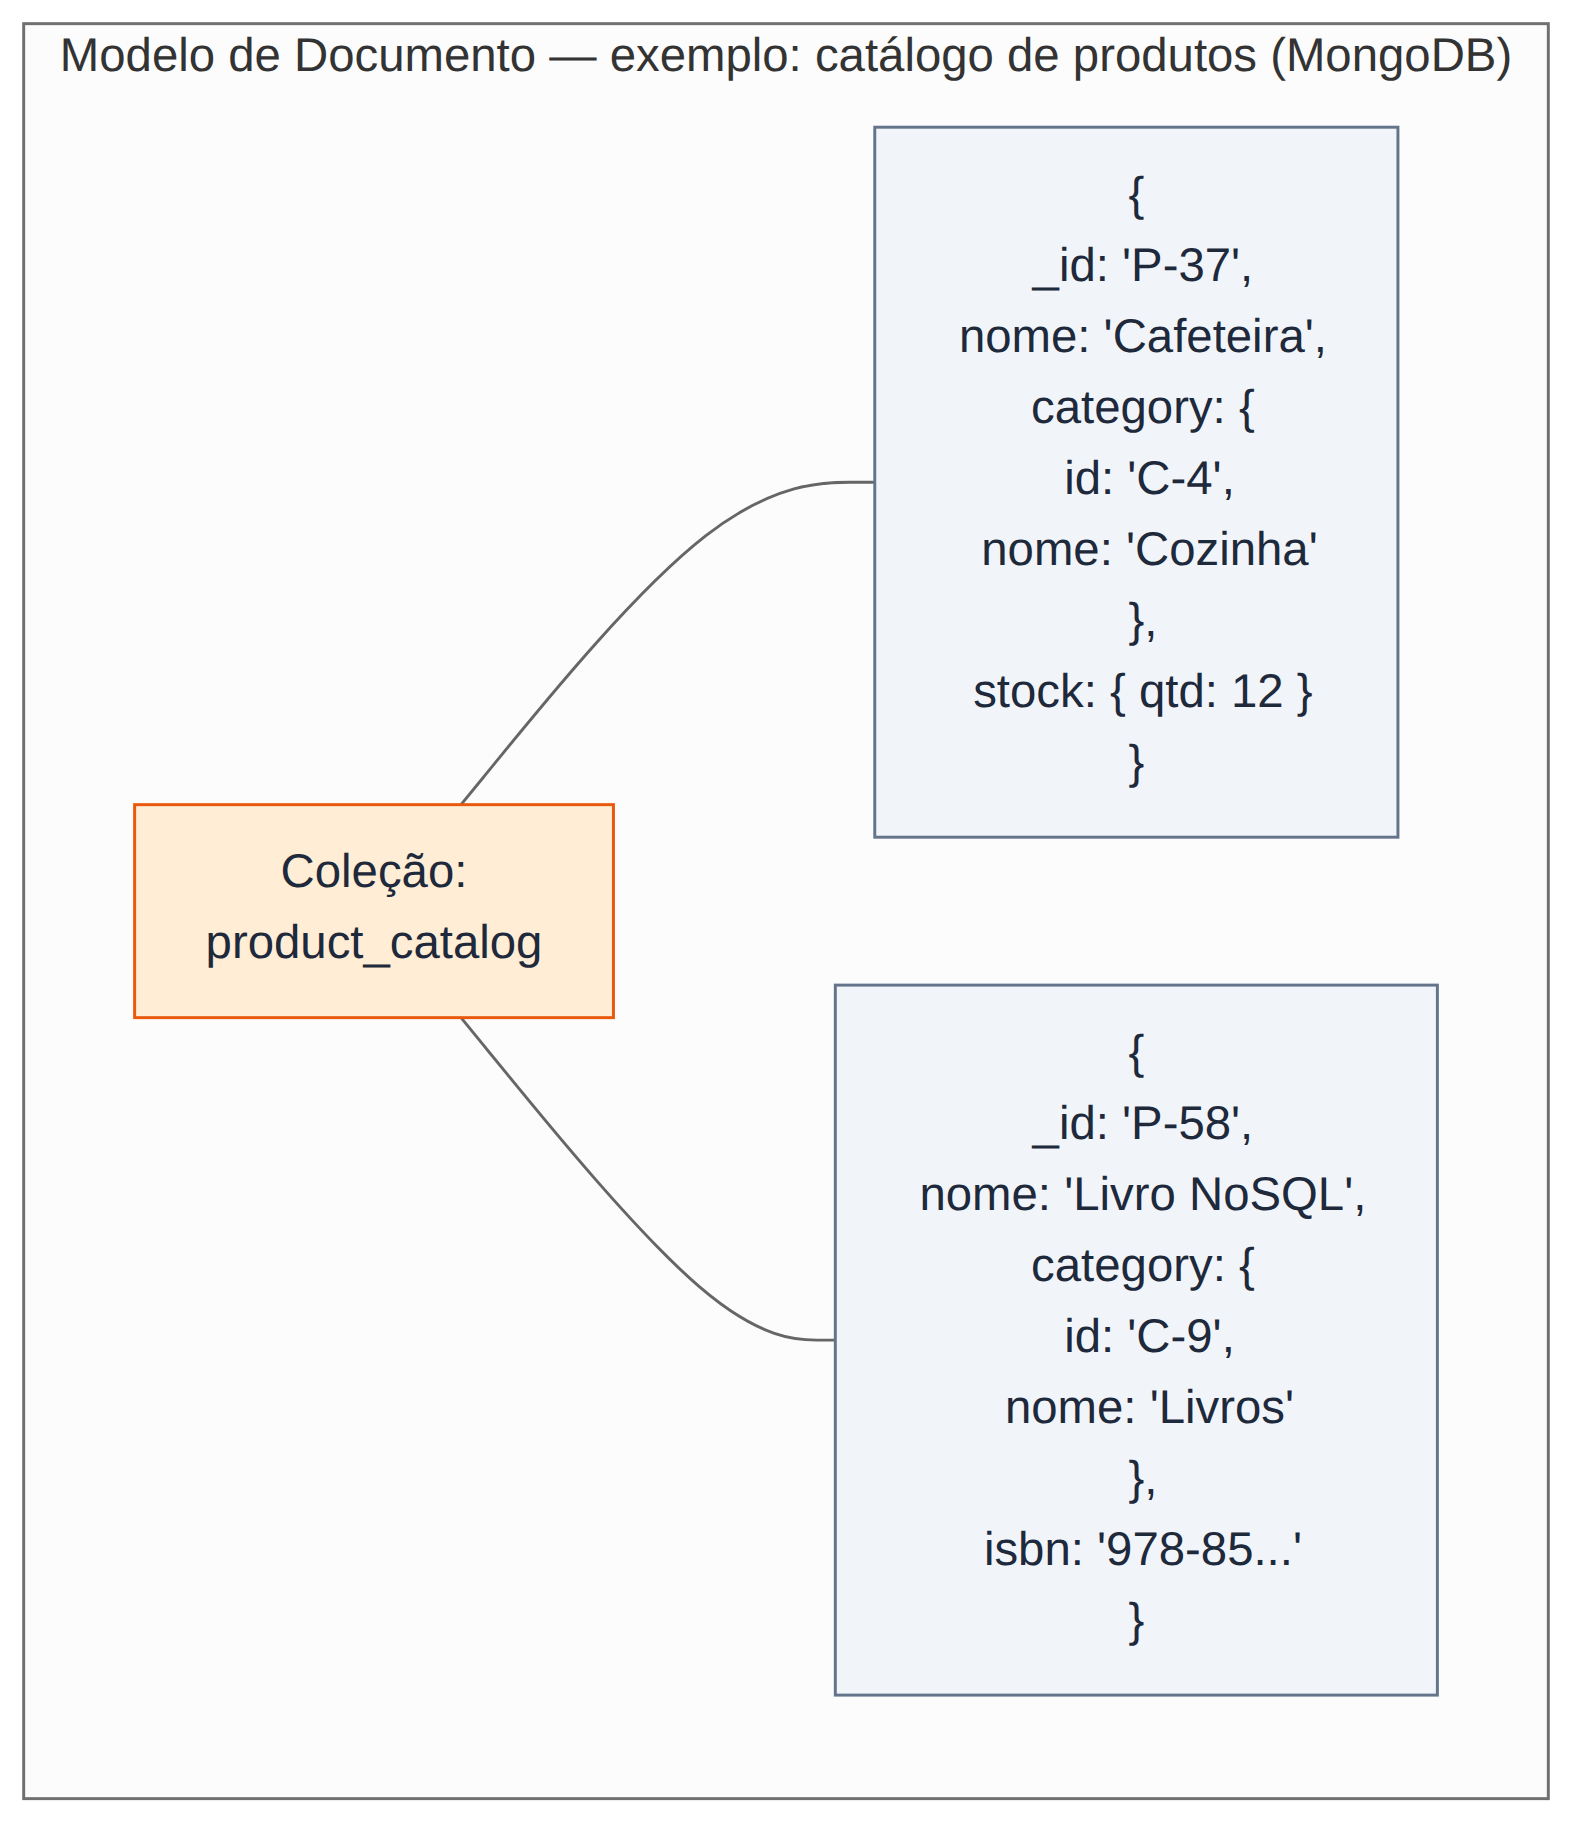
\includegraphics[width=10cm]{images/figure5-nosql-document}
  \par\vspace{4pt}
  {\footnotesize Fonte: Elaborado pelo autor (2026).}
\end{figure}

\subsection{Grafo}

Bancos de dados em grafo representam dados como \textbf{nós} (entidades) e \textbf{arestas}
(relacionamentos tipados), com propriedades em ambos. Consultas exploram caminhos e
vizinhanças de forma natural, o que é útil para recomendação, detecção de fraude e redes
sociais. O Neo4j utiliza a linguagem Cypher para \texttt{MERGE}/\texttt{CREATE} de nós e
relacionamentos.

Na ferramenta proposta, o destino grafo exige que o usuário declare explicitamente quais
colunas do CSV identificam cada rótulo de nó e quais colunas alimentam propriedades do
relacionamento (por exemplo, comprador $\rightarrow$ vendedor com atributos do pedido). A
Figura~\ref{fig:nosql-graph} exemplifica um cenário de recomendação, em que nós
\texttt{User} e \texttt{Product} são conectados por arestas tipadas (\texttt{PURCHASED},
\texttt{VIEWED}, \texttt{SIMILAR\_TO}), algumas portando propriedades próprias.

\begin{figure}[H]
  \centering
  \caption{Modelo de grafo: nós e arestas tipadas com propriedades (Neo4j).}
  \label{fig:nosql-graph}
  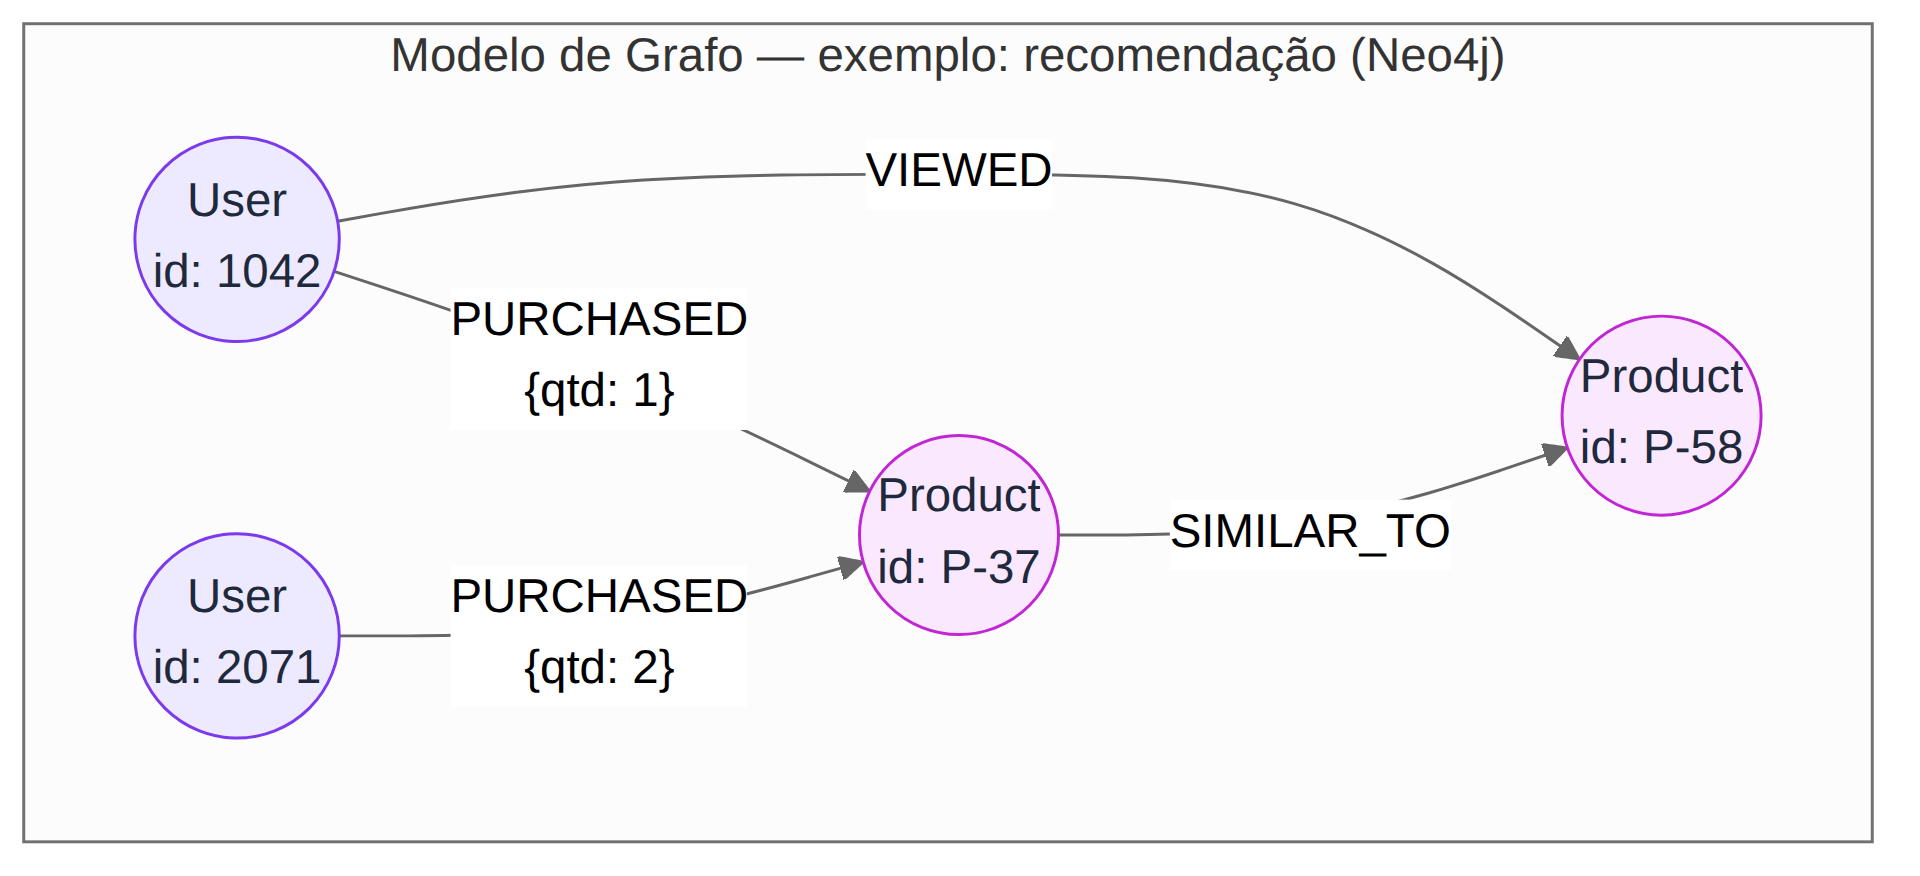
\includegraphics[width=13cm]{images/figure6-nosql-graph}
  \par\vspace{4pt}
  {\footnotesize Fonte: Elaborado pelo autor (2026).}
\end{figure}

\section{Bancos de Dados Multimodelo e Arquiteturas de Persistência Poliglota}

SGBDs multimodelo integram mais de um paradigma de dados no mesmo motor de gerência de
dados (por exemplo, documento + chave-valor + grafo), oferecendo em geral uma interface de
acesso unificada --- como a linguagem AQL do SGBD ArangoDB, que combina filtros sobre
estruturas de documento similares ao JSON e travessias em grafos em uma única abstração
de modelo de dados que combina ambos os modelos NoSQL.

A persistência poliglota, por outro lado, combina vários SGBDs heterogêneos, cada um
escolhido pela adequação a um caso de uso da aplicação \cite{sadalage2013nosql}. Na
literatura recente, essa ideia materializa-se como um SGPD (Sistema de Gerenciamento
Poliglota de Dados): coordenação transparente entre tecnologias distintas, com requisitos
de modelagem e expressividade de acesso (diferentes padrões de consulta) e capacidade de
adaptação quando o \textit{workload} evolui \cite{kiehn2022polyglot,glake2022towards}.

\citeonline{tan2017query} apresentam uma taxonomia útil para distinguir arquiteturas
relacionadas: BD federado (fontes homogêneas, interface única), BD multistore (fontes
heterogêneas, modelo canônico de consulta), BD \textit{polystore} (fontes heterogêneas,
múltiplas interfaces de acesso --- exemplificadas por sistemas como o BigDAWG) e
abordagens multimodelo (vários modelos no mesmo motor).

A escolha entre essas arquiteturas não é trivial. \citeonline{royhubara2022selecting}
propõem critérios para selecionar quais modelos de dados usar em aplicações de persistência
poliglota, destacando o \textit{trade-off} entre especialização por SGBD e simplicidade
operacional de um motor multimodelo.

O \textit{Polyglot Import CSV} adota explicitamente a linha da persistência poliglota ao
invés de multimodelo, conforme detalhado no capítulo 4. O usuário direciona entidades e
filtros para PostgreSQL, Redis, MongoDB, Cassandra e Neo4j conforme o padrão de
representação e acesso desejados.
